\section{等温管式反应器设计}


\begin{frame}
    \frametitle{活塞流模型管式反应器的设计方程}
    \begin{columns}[c]
        \column{2.6cm}
            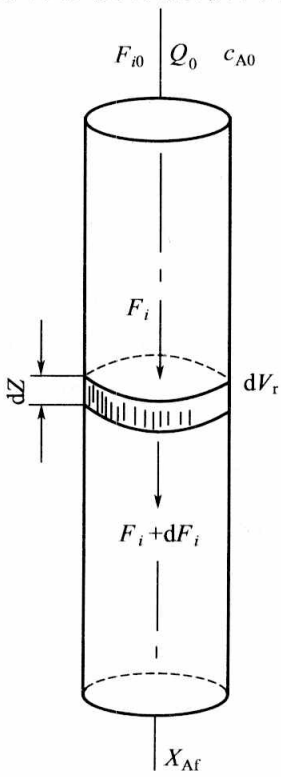
\includegraphics[width=\linewidth]{figs/fig4.2.png}
        \column{10.9cm}
            取微元体积$\mathrm{d}V_\mathrm{r}$作为控制体积，对此微元体作任意反应组分$i$的物料衡算，当过程达到定态时，
            \[
                F_{i}+\mathrm{d} F_{i}-F_{i}=\mathscr{R}_{i} d V_{\mathrm{r}}
            \]
            \[
                \frac{\mathrm{d} F_{i}}{d V_{\mathrm{r}}}=\mathscr{R}_{i}
            \]
    \end{columns}
\end{frame}


\begin{frame}
    \frametitle{物料衡算式}

    对于单一反应，只要对一个反应组分即关键组分作物料衡算就够了。
    \[
        \frac{\mathrm{d} F_{\mathrm{A}}}{d V_{\mathrm{r}}}=\mathscr{R}_{A}
    \]
    为计算反应体积，将$F_{\mathrm{A}}$与$\mathscr{R}_{A}$变为转化率的函数较为方便。
    
    将$F_{\mathrm{A}}=F_{\mathrm{A0}}(1-X_{\mathrm{A}})$代入，得
    \[
        F_{\mathrm{A} 0} \frac{\mathrm{d} X_{\mathrm{A}}}{\mathrm{d} V_{\mathrm{r}}}=-\mathscr{R}_{\mathrm{A}}(X_{\mathrm{A}})
    \]
    因$F_{\mathrm{A0}}=Q_0 c_{\mathrm{A0}}$，上式又可写成
    \[
        Q_0 c_{\mathrm{A0}} \frac{\mathrm{d} X_{\mathrm{A}}}{\mathrm{d} V_{\mathrm{r}}}=-\mathscr{R}_{\mathrm{A}}(X_{\mathrm{A}})
    \]
    以上均为管式反应器的设计方程，实际应用时可根据具体情况选定。

\end{frame}


\begin{frame}
    \frametitle{反应体积的计算}

    积分管式反应器设计方程可得反应体积
    \[
        V_{\mathrm{r}}=Q_{0} c_{\mathrm{A} 0} \int_{0}^{X_{\mathrm{Af}}} \frac{\mathrm{d} X_{\mathrm{A}}}{[-\mathscr{R}_{\mathrm{A}}(X_{\mathrm{A}})]}
    \]
    如果反应系以等速率进行，则$\mathscr{R}_{\mathrm{A}}$为常数，上式可化为
    \[
        V_{\mathrm{r}}=\frac{Q_{0} c_{\mathrm{A} 0} X_{\mathrm{Af}}}{-\mathscr{R}_{\mathrm{A}}(X_{\mathrm{Af}})}
    \]
    \begin{columns}[c]
        \column{6.5cm}        
        \[
            \text{空时}~~~\quad \tau=c_{\mathrm{A} 0} \int_{0}^{X_{\mathrm{Af}}} \frac{\mathrm{d} X_{\mathrm{A}}}{[-\mathscr{R}_{\mathrm{A}}\left(X_{\mathrm{A}}\right)]} 
        \]
        间歇釜式反应器的反应时间
        \[
            t=c_{\mathrm{A} 0} \int_{0}^{X_{\mathrm{Af}}} \frac{\mathrm{d} X_{\mathrm{A}}}{[-\mathscr{R}_{\mathrm{A}}\left(X_{\mathrm{A}}\right)]} 
        \]
        \column{7cm}
            \begin{itemize}
                \item[\bullet] 等容下反应，$\tau=t$
                \item[\bullet] 变容下反应，$\tau \neq t$
            \end{itemize}
    \end{columns}
\end{frame}


\begin{frame}
    \frametitle{轴向浓度分布}

    设$u_0$为反应器进口处流体的流速，可写成转化率与轴向距离$Z$的关系式
    \[
        u_0 c_{\mathrm{A0}} \frac{\mathrm{d} X_{\mathrm{A}}}{\mathrm{d} Z}=-\mathscr{R}_{\mathrm{A}}(X_{\mathrm{A}})
    \]
    若为等容过程，可写成轴向浓度分布方程
    \[
        u_0 \frac{\mathrm{d} c_{\mathrm{A}}}{\mathrm{d} Z}=\mathscr{R}_{\mathrm{A}}
    \]
    可看出，对于定态操作的活塞流反应器，反应物系的浓度系随轴向距离而变，与时间无关。

    而间歇釜式反应器反应物系的浓度则随时间而变，与位置无关。
    \[
        \frac{\mathrm{d} c_{\mathrm{A}}}{\mathrm{d} t}=\mathscr{R}_{\mathrm{A}}
    \]

\end{frame}


\begin{frame}
    \frametitle{}

    \begin{example}
        采用活塞流管式反应器，等温下进行某均相反应\ch{A -> B}，$r_\mathrm{A}=5.2c_\mathrm{A}$ (\si{mol.L^{-1}.h^{-1}})，每天生产B 20kmol，A的初始浓度为2mol/L，最终转化率为80\%。计算总反应体积。
    \end{example}
    \pause
    \[
        Q_0 = \frac{20000}{24\times 0.8 \times 2} = 520.8 \mathrm{L}
    \]
    \[
        \tau =\frac{1}{k}\ln \frac{1}{1-X_{\mathrm{A}}}=\frac{1}{5.2}\ln \frac{1}{1-0.8}=0.3095 \mathrm{h}
    \]
    \[
        V_{\mathrm{r}}=Q_{0}\tau = 520.8 \times 0.3095 = 161.2 \mathrm{L}
    \]
    \pause 
    \vspace{-1em}
    \begin{table}
        \begin{tabular}{|c|c|c|c|}
            \hline
            间歇釜 $(t_0=0.25\mathrm{h})$ & 连续釜 & 双釜串联 & 管式反应器\\
            \hline
            292 L & 401 L & 247.6 L & 161.2 L\\
            \hline
        \end{tabular}
    \end{table}

\end{frame}

\begin{frame}
    \frametitle{多个反应}

    当反应器同时进行数个反应时，一个反应变量的变化已不足以描述整个反应过程。与釜式反应器一样，需分别对各关键组分作物料衡算，以获得管式反应器的设计方程组。作法与单一反应的情况完全一样，只是方程数目增加而已。
    \[
        \frac{\mathrm{d} F_{i}}{\mathrm{~d} V_{\mathrm{r}}}=\mathscr{R}_{i} \qquad(i=1,2, \cdots, K)
    \]
    对于等容过程，可选择任何形式的反应变量，但变容过程则以选$F_{i}$作为反应变量较为方便。由于N个反应组分并非都是关键组分，这就需将非关键组分的摩尔流量变为关键组分摩尔流量的函数。

    对于等容过程，应用下两个式子可能要方便些。
    \[
       Q_0\frac{\mathrm{d} c_{i}}{\mathrm{~d} V_{\mathrm{r}}}=\mathscr{R}_{i} \quad \text{或} \quad u_0\frac{\mathrm{d} c_{i}}{\mathrm{~d} Z}=\mathscr{R}_{i} \qquad(i=1,2, \cdots, K)
    \]

\end{frame}


\begin{frame}[t]
    \frametitle{}

    \begin{example}
        气体A$_1$与A$_2$在等温活塞流反应器中等压下进行下列气相反应
        \[\begin{array}{ll}
            2 \mathrm{~A}_{1}+\mathrm{A}_{2} \longrightarrow \mathrm{A}_{3} & \bar{r}_1=k_{1} c_{1}^{2} c_{2} \\
            \mathrm{~A}_{3}+\mathrm{A}_{2} \longrightarrow \mathrm{A}_{4} & \bar{r}_2=k_{2} c_{3} c_{2} \\
            2 \mathrm{~A}_{4} \longrightarrow \mathrm{A}_{5} & \bar{r}_3=k_{3} c_{4}^{2}
            \end{array}
        \]
        以$F_i$及$V_\mathrm{r}$为变量，列出反应器的设计方程。假定进料中不含反应产物。
    \end{example}

\end{frame}


\begin{frame}[t]
    \frametitle{}
    \begin{example}
        在管式反应器中于4.05 MPa 及 936 K 等温下进行三甲基萘脱烷基反应：
        \[
            \begin{aligned}
                \ch{T + H2 -> D + CH4}  \qquad r_1 &= k_1c_\mathrm{T}c_\mathrm{H}^{0.5} \quad \si{kmol.m^{-3}.s^{-1}}\\
                \ch{D + H2 -> M + CH4}  \qquad r_2 &= k_2c_\mathrm{D}c_\mathrm{H}^{0.5} \quad \si{kmol.m^{-3}.s^{-1}}\\
                \ch{M + H2 <=> N + CH4}  \qquad r_3 &= \vec{k_3}(c_\mathrm{M}c_\mathrm{H}^{0.5}-c_\mathrm{N}c_\mathrm{G}/c_\mathrm{H}^{0.5}K) \quad \si{kmol.m^{-3}.s^{-1}}
            \end{aligned}
        \]
        下标 T 、 D 、 M 、 H 、 G 及 N 分别代表三甲基萘 、 二甲基萘 、 一甲基萘 、 氢 、 甲烷及萘 。反应温度下，$k_1=5.66\times 10^{-6}$，$k_2=5.866\times 10^{-6}$，$\vec{k_3}=2.052\times 10^{-6}$，$K=5$。原料气组成的摩尔分数三甲基萘为 25\% ， 氢 75\% ， 在操作温度及压力
        下 ， 以 0.1 m/s 的流速送入反应器 ， 要求三甲基萘的转化率达 80\% ， 试计算 ：
        
        (1) 所需的反应器长度 ；
        
        (2) 二甲基萘 、 一甲基萘及萘的收率 。
    \end{example}
\end{frame}


\begin{frame}
    \frametitle{多相催化反应模型的建立}

    多相催化反应过程中，化学反应系在固体催化剂的表面上发生，流体相中的反应物需向固体催化剂表面上传递，生成的反应产物又需作反方向传递。与化学反应进行的同时必然产生一定的热效应，于是固体催化剂与流体间还存在着热量传递。那么，固体催化剂上反应组分的浓度与流体相将是不同的；固体催化剂的温度也与流体的温度不同。如果两者间的传质和传热的速率很大，则两者的浓度及温度的差异将很小。虽为多相催化反应，若忽略这些差异，则在动力学表征上与均相反应并无两样。所以，根据这种简化假定而建立的模型称为拟均相模型。

\end{frame}


\begin{frame}
    \frametitle{拟均相模型}

    在管式反应器中进行多相催化反应时，如果符合拟均相假定，则前面所导出的各种式子同样适用。但应注意，反应体积$V_\mathrm{r}$对均相反应而言指的是进行化学反应的空间，对多相催化反应则为催化剂的堆体积，即催化剂颗粒本身的体积加上颗粒与颗粒间的空隙体积。
    
    若基于催化剂的质量来表示反应速率，则
    \[
        \frac{\mathrm{d} F_{i}}{\mathrm{~d} V_{\mathrm{r}}}=\rho_\mathrm{b} \mathscr{R}_{i} \qquad(i=1,2, \cdots, K)
    \]
    式中，$\rho_\mathrm{b}$为催化剂的堆密度。上式又可改写成
    \[
        \frac{\mathrm{d} F_{i}}{\mathrm{~d} W}=\mathscr{R}_{i} \qquad(i=1,2, \cdots, K)
    \]

\end{frame}


\begin{frame}[t]
    \frametitle{}

    \begin{example}
        在277℃，\SI{1.103e5}{Pa}压力下在活塞流反应器进行气固相催化反应
        \[
            \ch{C2H5OH + CH3COOH -> CH3COOC2H5 + H2O}
        \]
        \[
            (A)\qquad \qquad (B)\qquad \qquad \quad (P) \qquad \qquad (Q)
        \]
        催化剂的堆密度为\SI{700}{kg/m^3}。该温度下B的转化速率为
        \[
            r_{B}=\frac{4.096 \times 10^{-7}(0.3+8.885 \times 10^{-6} p_{Q})(p_{B}-p_{P} p_{Q} / 9.8 p_{A})}{3600(1+1.515 \times 10^{-4} p_{p})} \qquad \si{kmol/(kg.s)}
        \]
        式中的分压以Pa表示，假定气固两相间的传质阻力可忽略不计。加料组成为23\%B，46\%A，31\%Q（均为重量\%），加料中不含酯，当$X_\mathrm{B}=35\%$时，所需的催化剂量是多少？反应体积是多少？乙酸乙酯的产量为2083kg/h。

    \end{example}

\end{frame}